\section{Przetwornik C/A}
Wykorzystując płytkę UA-1 zmontowano sumator o trzech wieściach \(U_1\), \(U_2\) i \(U_3\) (Rys. \ref{sh2}). Wyjścia sumatora odwzorowują 3 bity binarnej reprezentacji liczby \(X\)
Do budowy wybrano rezystory \(R=33k\) (5\%).
Następnie na wejścia sumatora reprezentujące bity \(X_1\), \(X_2\) oraz \(X_3\) podawano napięcie \(0V\) lub \(U_p\approx1V\) (za pomocą rezystora nastawnego), mierząc przy tym napięcia \(U_{wy}\) i \(U_p\).
Pomiary przeprowadzono dla \(X\) od 0 do 7, wyniki umieszczono w Tab. \ref{tab1}.
Zaobserwowana nieliniowość przetwornika może wynikać z niedokładności wykonania rezystorów oraz błędów pomiarowych, obliczony współczynnik proporcjonalności uwzględnia spadek napięcia \(U_p\).

\begin{figure}[H]
	\centering
	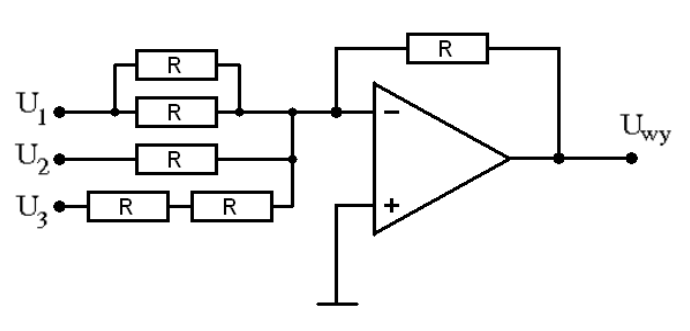
\includegraphics[width=11cm]{include/2/1.png}
	\caption{Schemat zbudowanego układu.}
	\label{sh2}
\end{figure}

\begin{table}[H]
	\centering
	\begin{tabular}{c|c c c|c||c|c}
		\hline
		\(X\) & \(X_1\) & \(X_2\) & \(X_3\) & \(U_p\)[V] & \(U_{wy}\)[V] & \(\frac{X}{U_{wy}} U_p\) \\ \hline\hline
		0     & 0       & 0       & 0       & 1.004      & 0.001         & \(n/a\)                  \\ \hline
		1     & 0       & 0       & 1       & 0.991      & -0.493        & -2.010                   \\ \hline
		2     & 0       & 1       & 0       & 0.978      & -0.993        & -1.969                   \\ \hline
		3     & 0       & 1       & 1       & 0.966      & -1.465        & -1.978                   \\ \hline
		4     & 1       & 0       & 0       & 0.954      & -1.927        & -1.980                   \\ \hline
		5     & 1       & 0       & 1       & 0.943      & -2.377        & -1.983                   \\ \hline
		6     & 1       & 1       & 0       & 0.931      & -2.828        & -1.975                   \\ \hline
		7     & 1       & 1       & 1       & 0.920      & -3.257        & -1.977                   \\ \hline
	\end{tabular}
	\caption{Pomiar napięcia wyjściowego \(U_{wy}\) oraz napięcia wejściowego (na potencjometrze) \(U_p\), dla \(X\) od 0 do 7}
	\label{tab1}
\end{table}
